% !TEX root = ../main.tex
\chapter{Моделювання замкнених систем}
Користуючись рівнянням \eqref{PID:pos_alg}, проведемо моделювання замкнених систем з різними
передаточними функціями об'єкта.

\section{Випадок 
\texorpdfstring{$W_O(s) = \frac{ k e^{-\tau s}}{(T_1 s + 1) (T_2 s + 1) (T_3 s + 1)}$}{1}}
Оптимальні настройки регулятора було обчислено в пункті \ref{sec:resonance_3rd_order}.
Зв'язок між вихідною координатою та керуючим діянням задається диференціальним рівнянням
\begin{gather*}
    \mbox{\normalsize 
    $T_1 T_2 T_3 \frac{d^3 y(t)}{dt^3} +
    \left(T_1 T_2 + T_1 T_3 + T_2 T_3 \right) \frac{d^2 y(t)}{dt^2} + 
    \left(T_1 + T_2 + T_3 \right) \frac{d y(t)}{dt} + y(t) = k u(t-\tau)$}
\end{gather*}
Перехідний процес при подачі на задаюче діяння одиничного імпульсу:
\begin{center}
    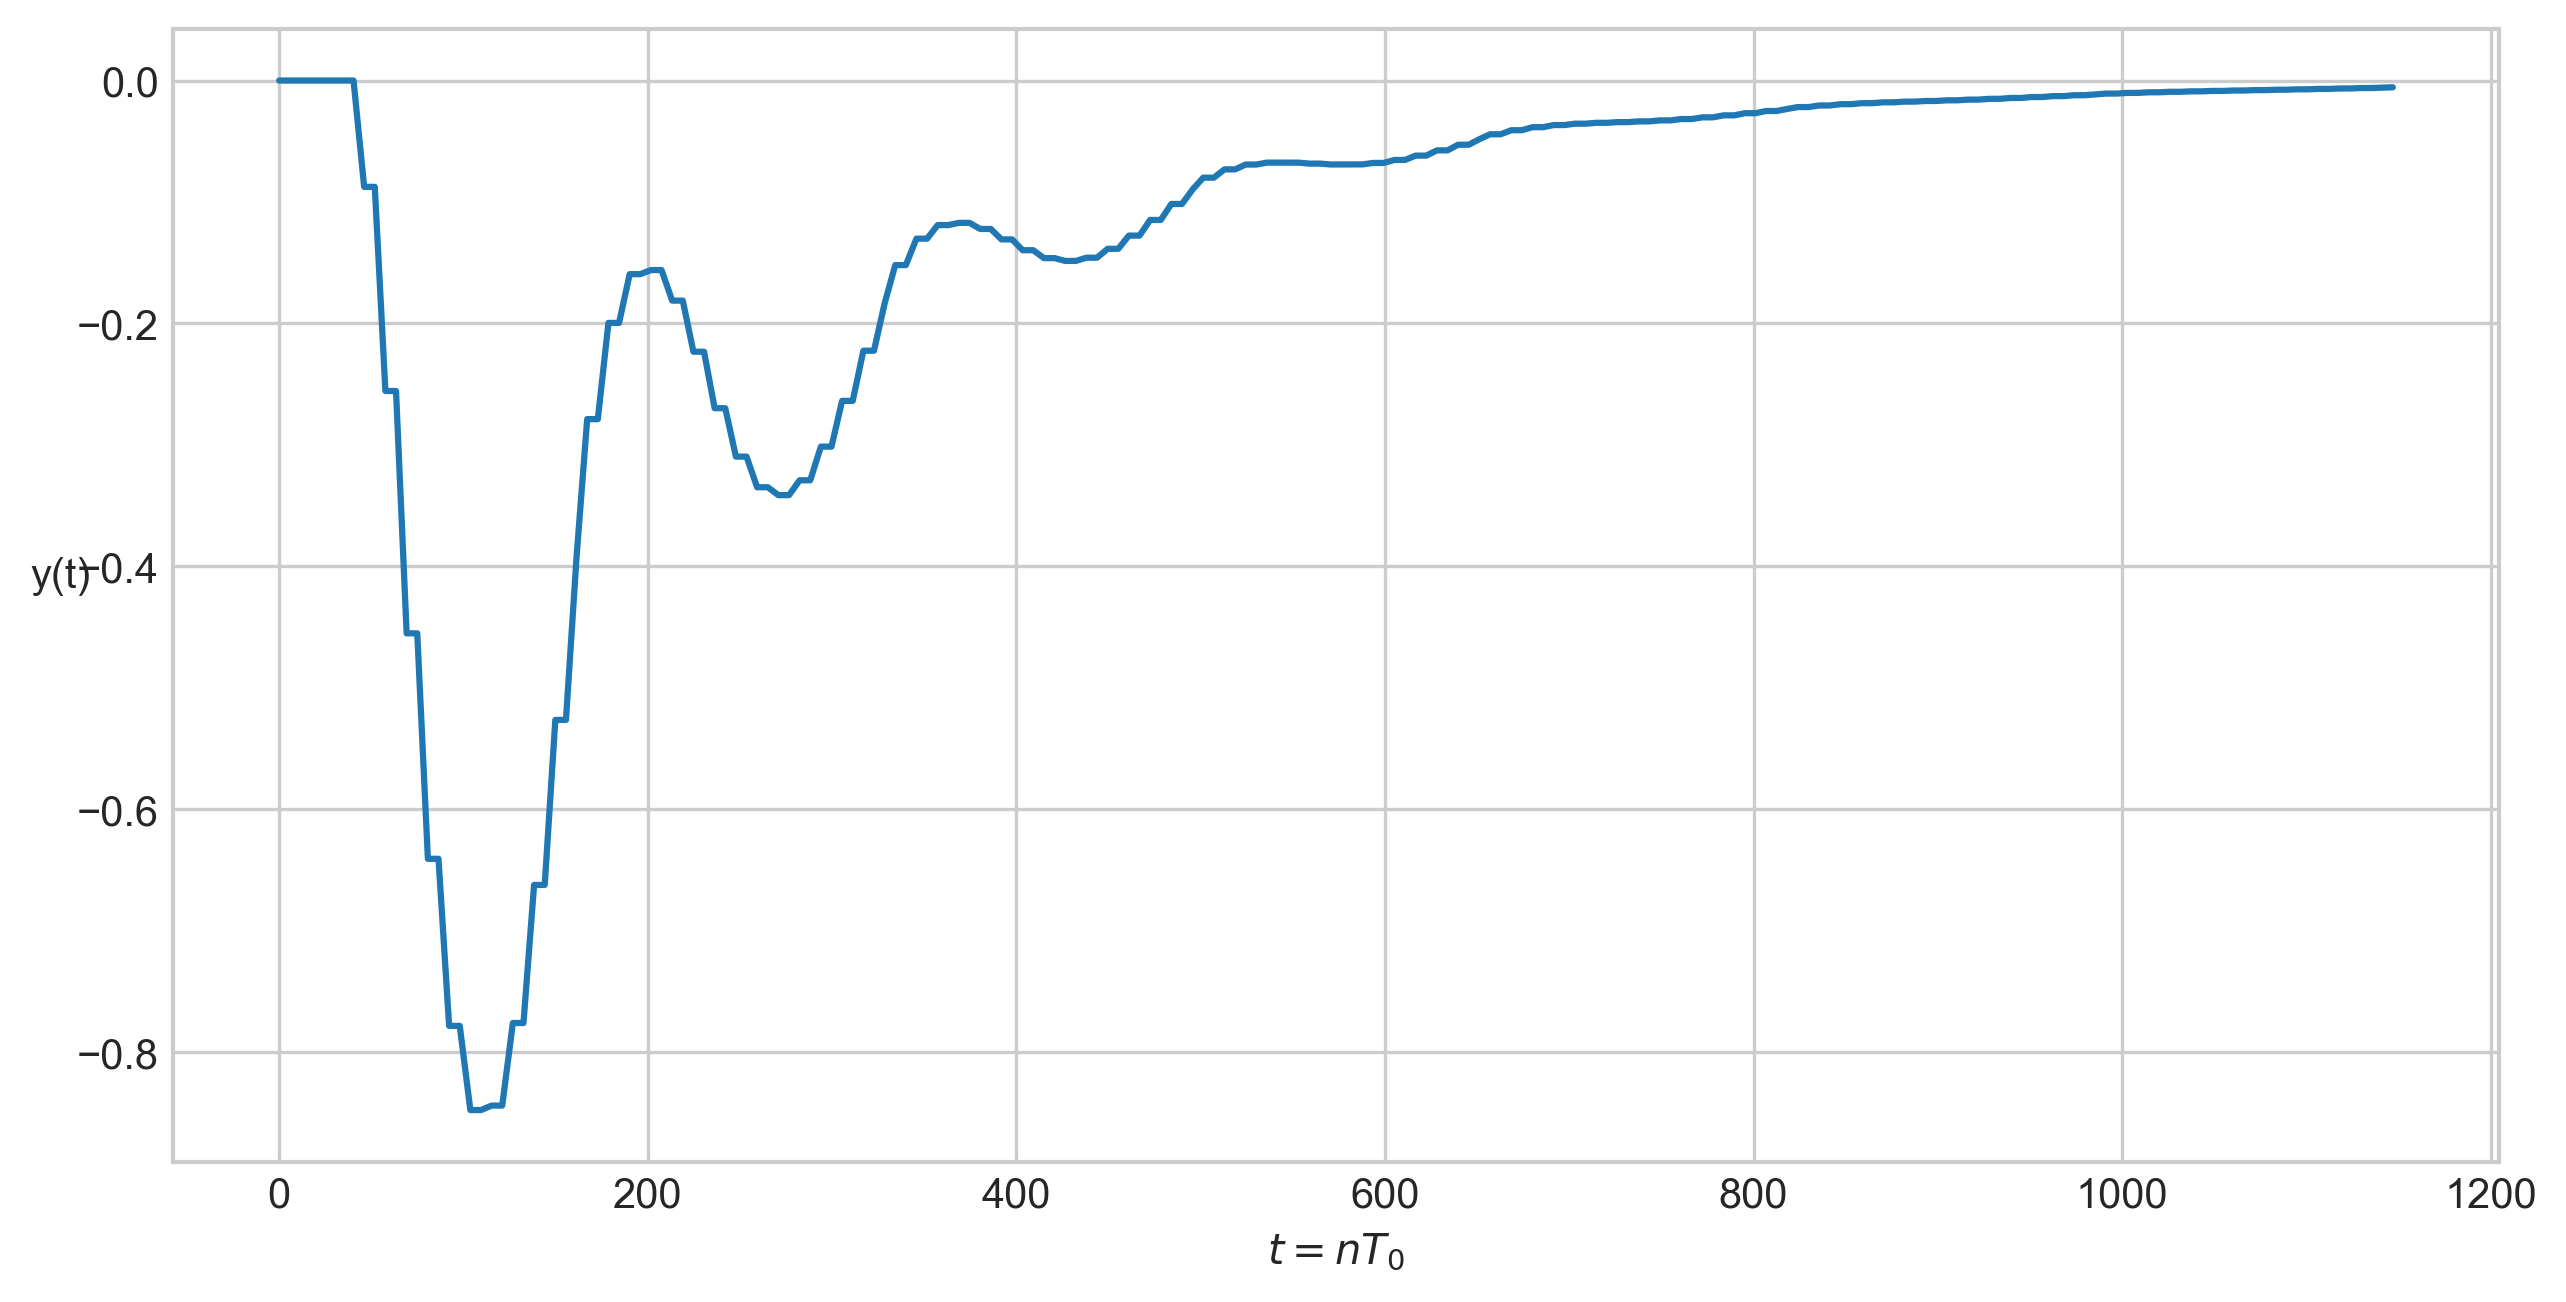
\includegraphics[width=\textwidth]{pics/transient_process_final_9_1_impulse.png}
\end{center}
% Перехідний процес при подачі на задаюче діяння одиничного ступінчатого збурення:
% \begin{center}
%     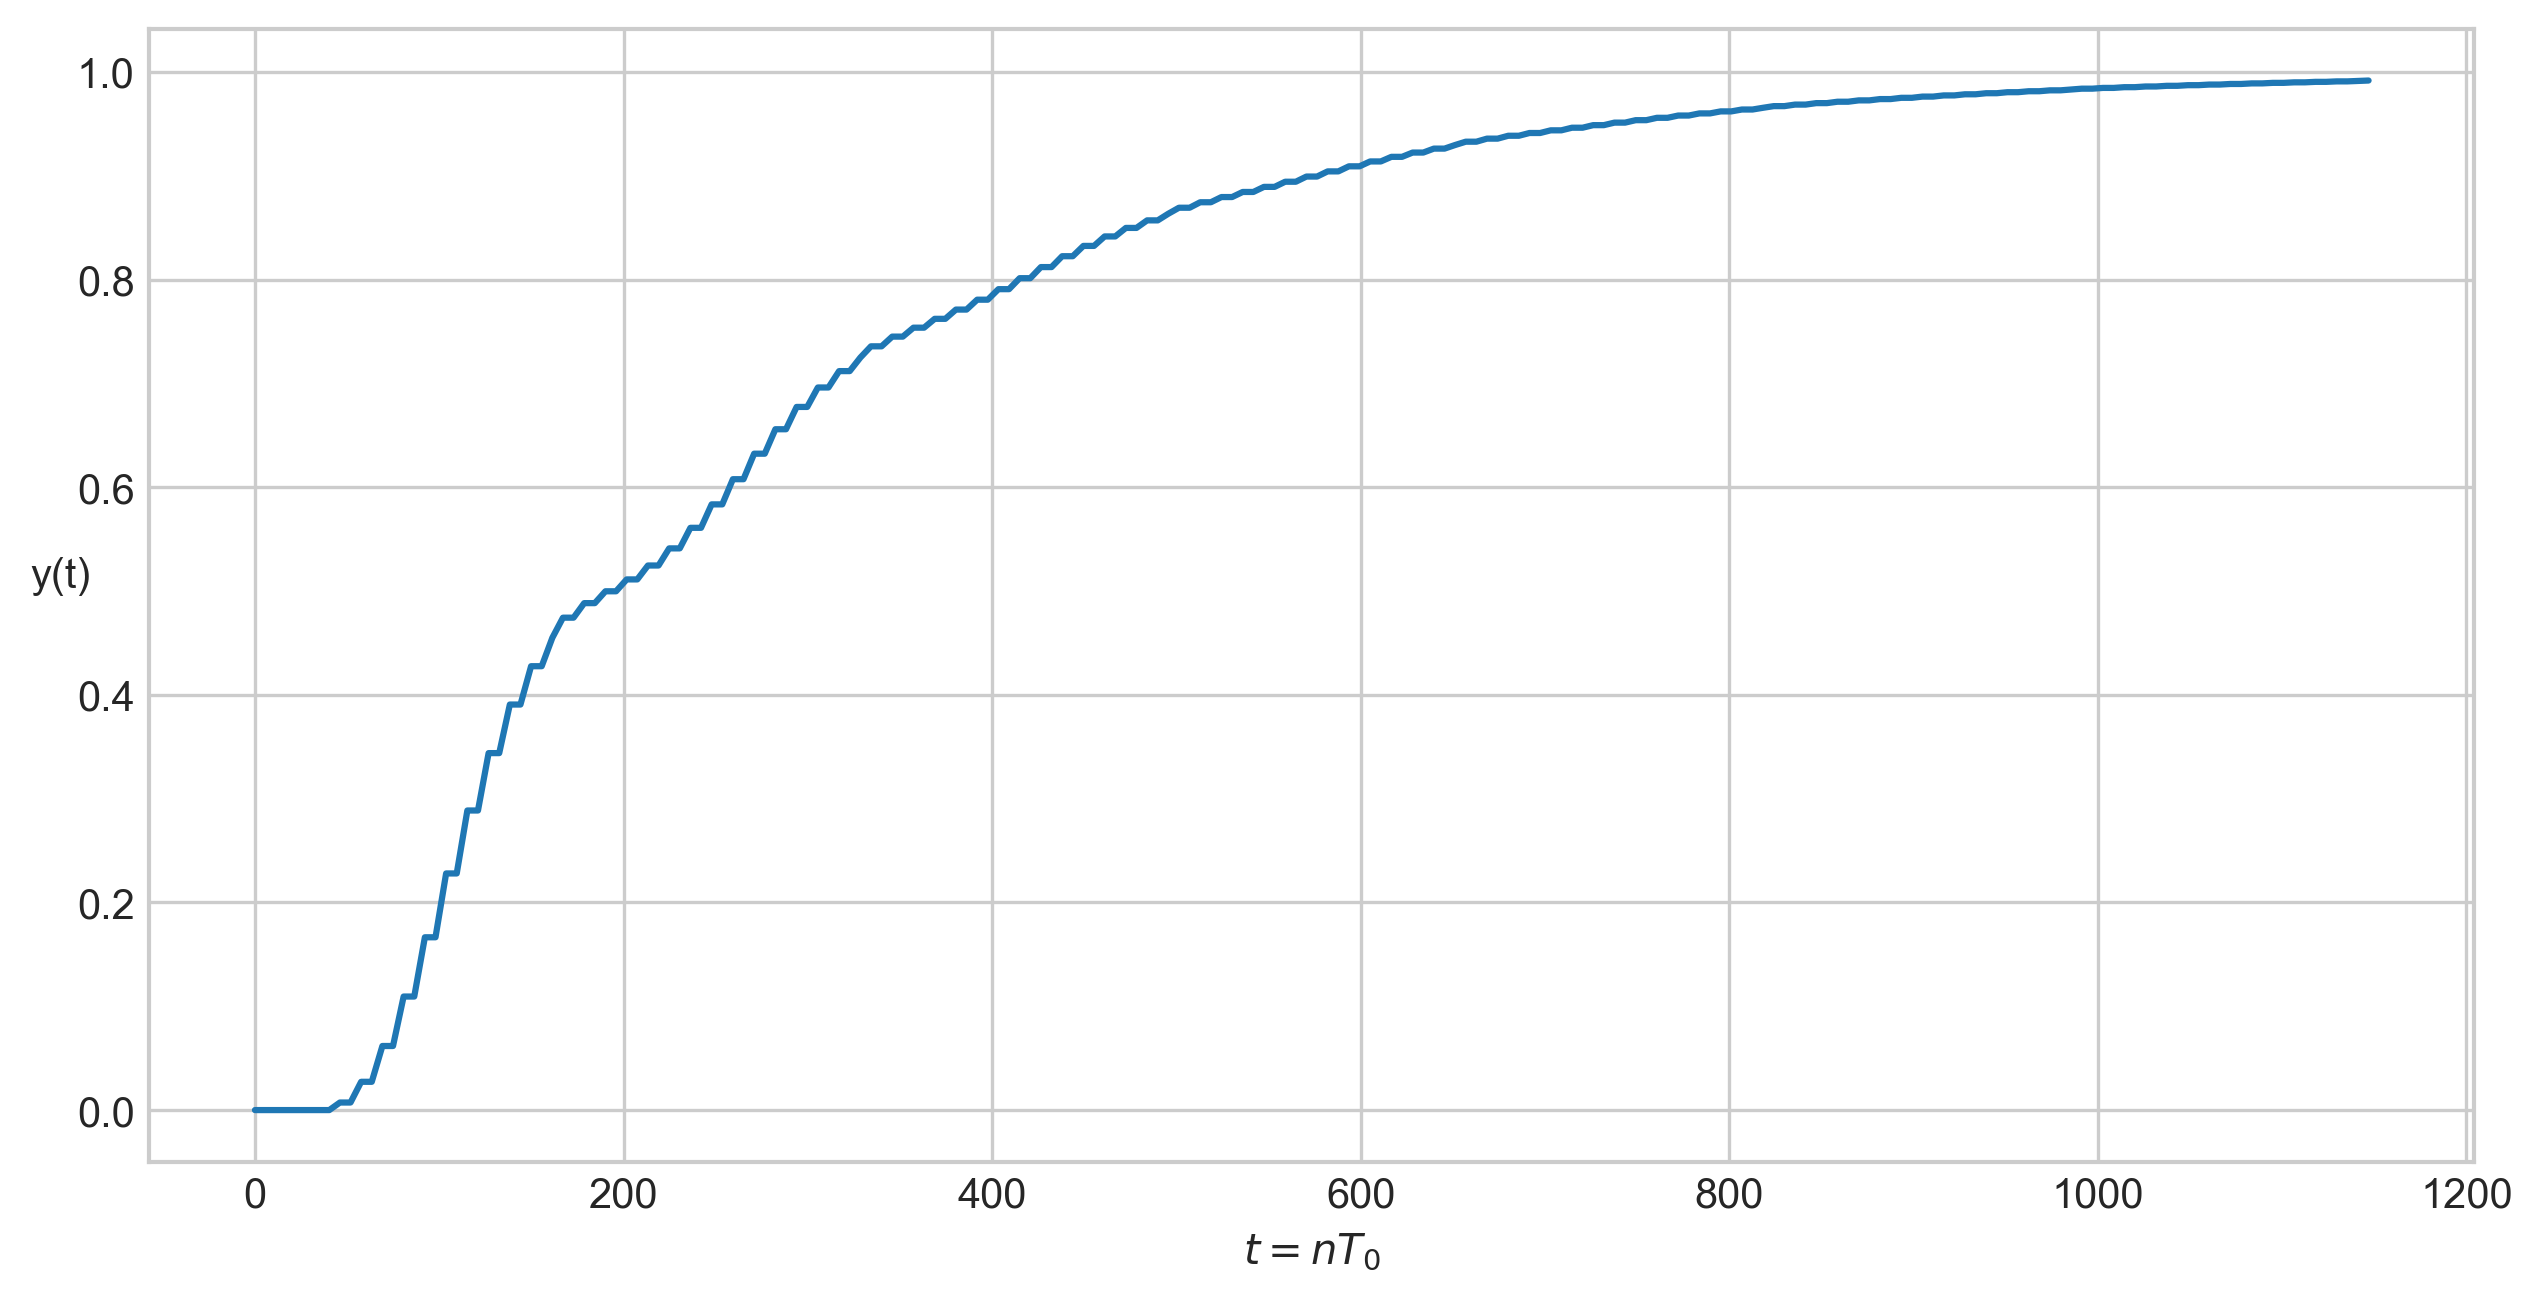
\includegraphics[scale=0.7]{pics/transient_process_final_9_1_step.png}
% \end{center}

\section{Випадок 
\texorpdfstring{$W_O(s) = \frac{ k e^{-\tau s}}{(T_1 s + 1) (T_2 s + 1)}$}{1}}
Оптимальні настройки регулятора було обчислено в пункті \ref{sec:resonance_2nd_order}.
Зв'язок між вихідною координатою та керуючим діянням задається диференціальним рівнянням
\begin{gather*}
    \mbox{\normalsize 
    $T_1 T_2 \frac{d^2 y(t)}{dt^2} +
    \left(T_1 + T_2 \right) \frac{d y(t)}{dt} + y(t) = k u(t-\tau)$}
\end{gather*}
Перехідний процес при подачі на задаюче діяння одиничного імпульсу:
\begin{center}
    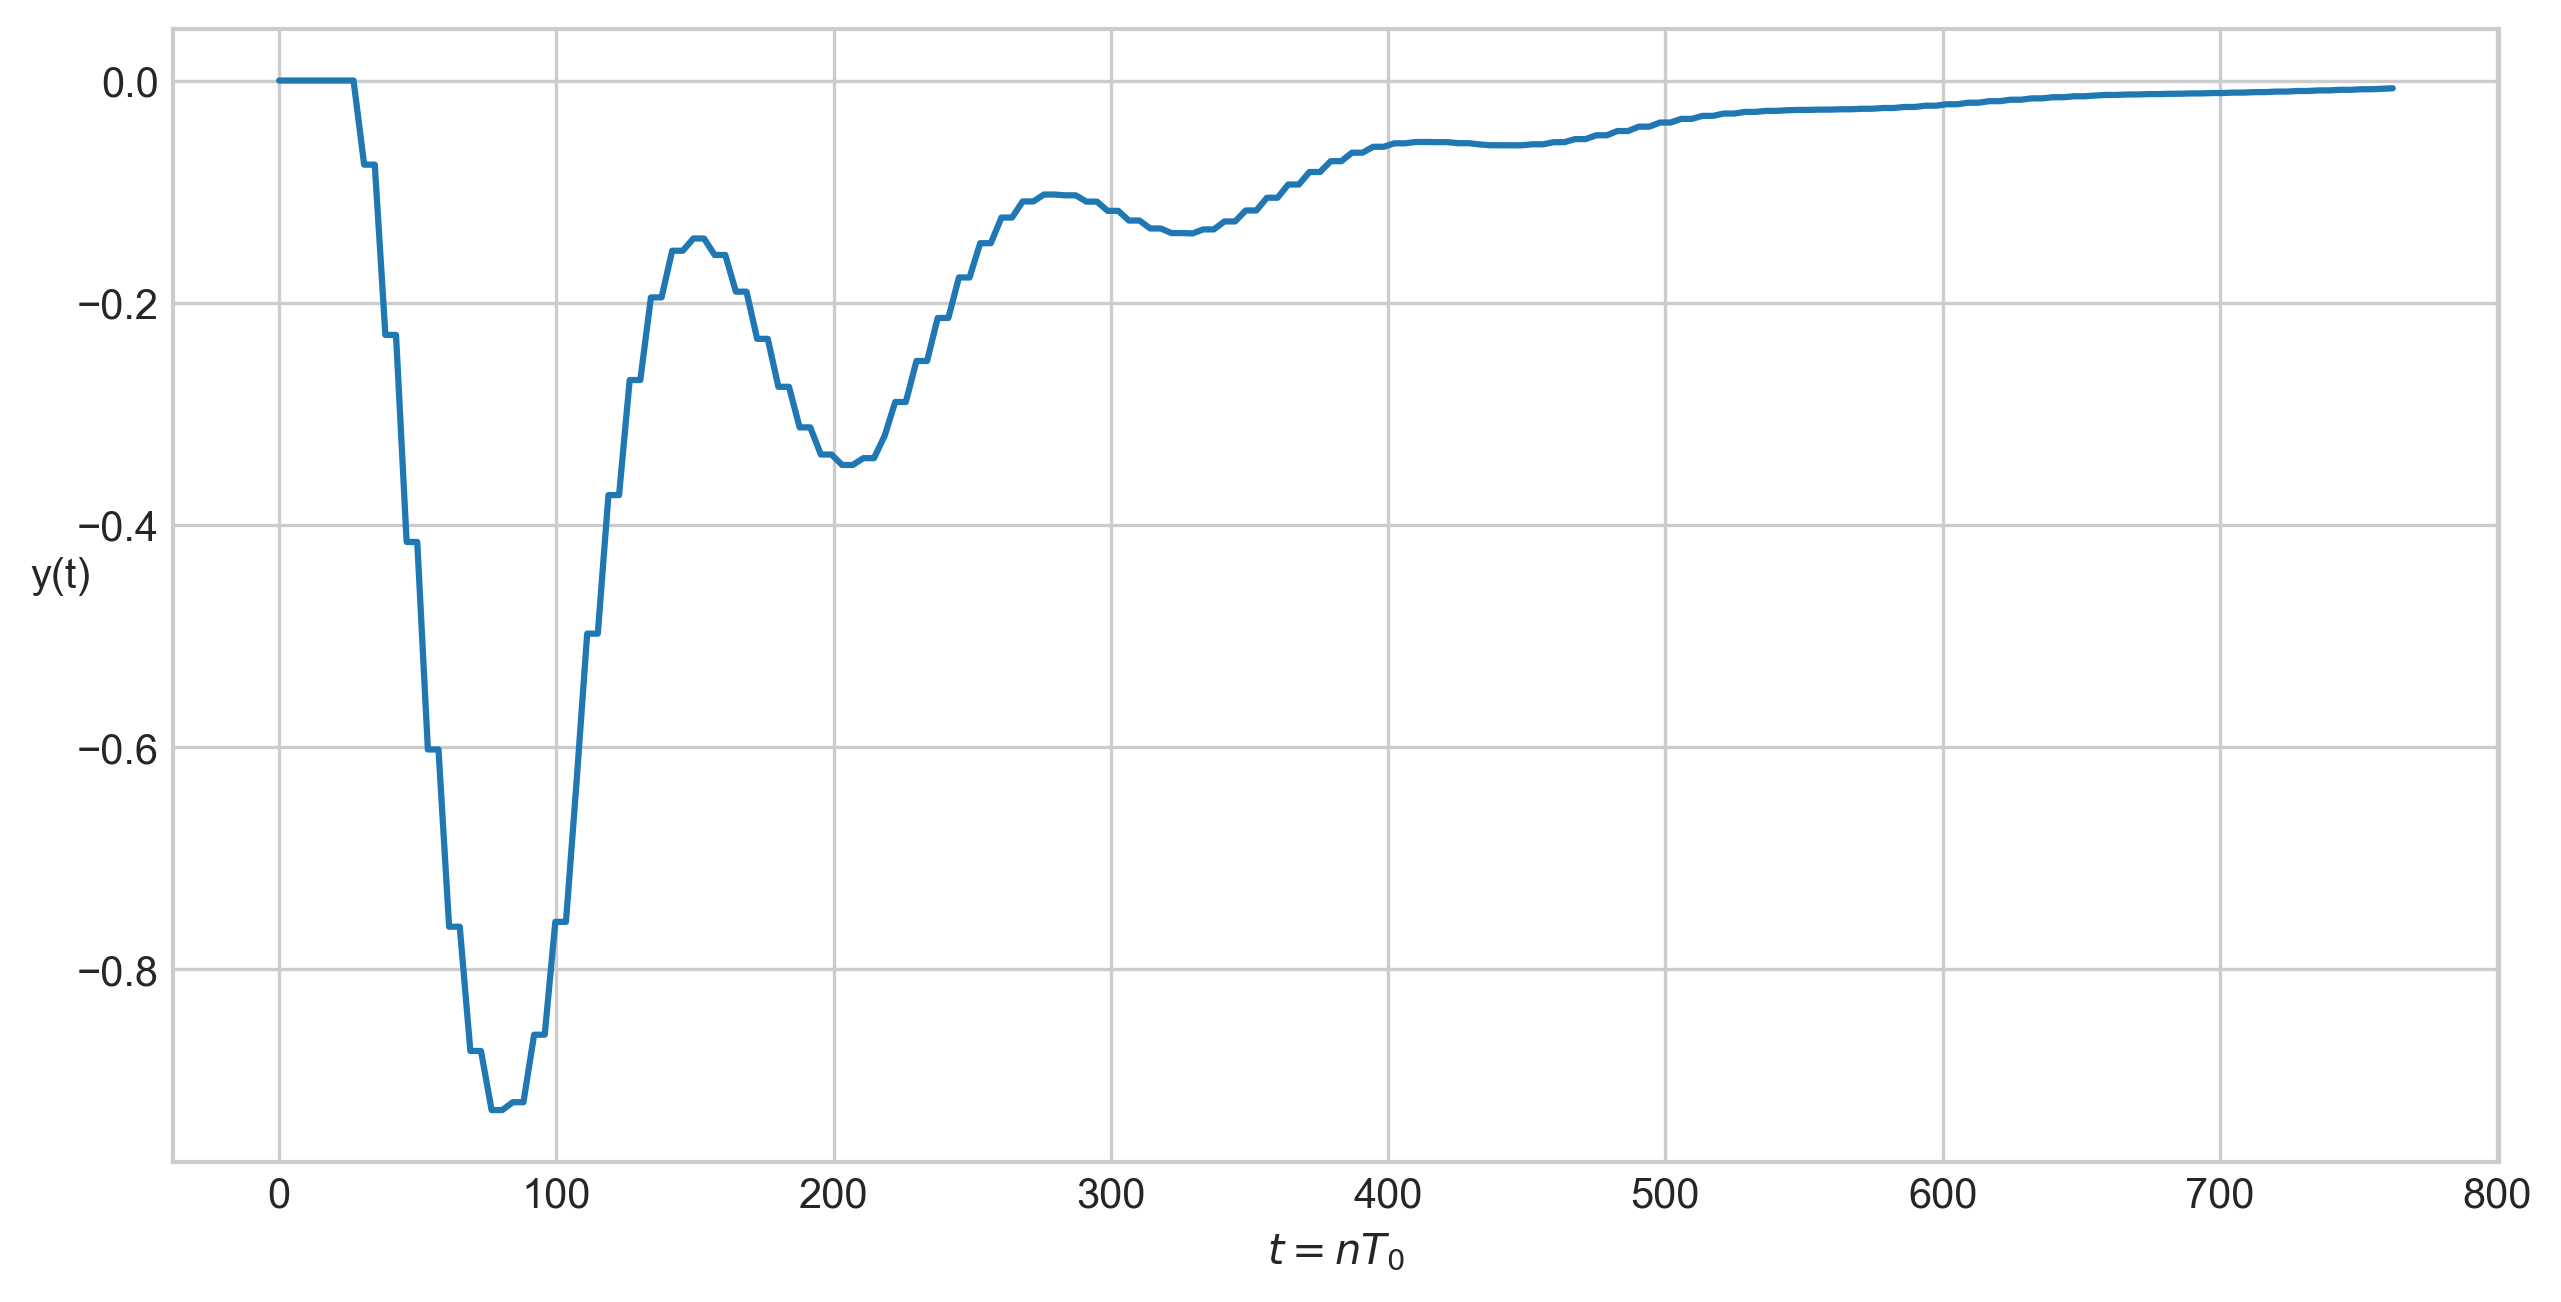
\includegraphics[width=\textwidth]{pics/transient_process_final_9_2_impulse.png}
\end{center}
% Перехідний процес при подачі на задаюче діяння одиничного ступінчатого збурення:
% \begin{center}
%     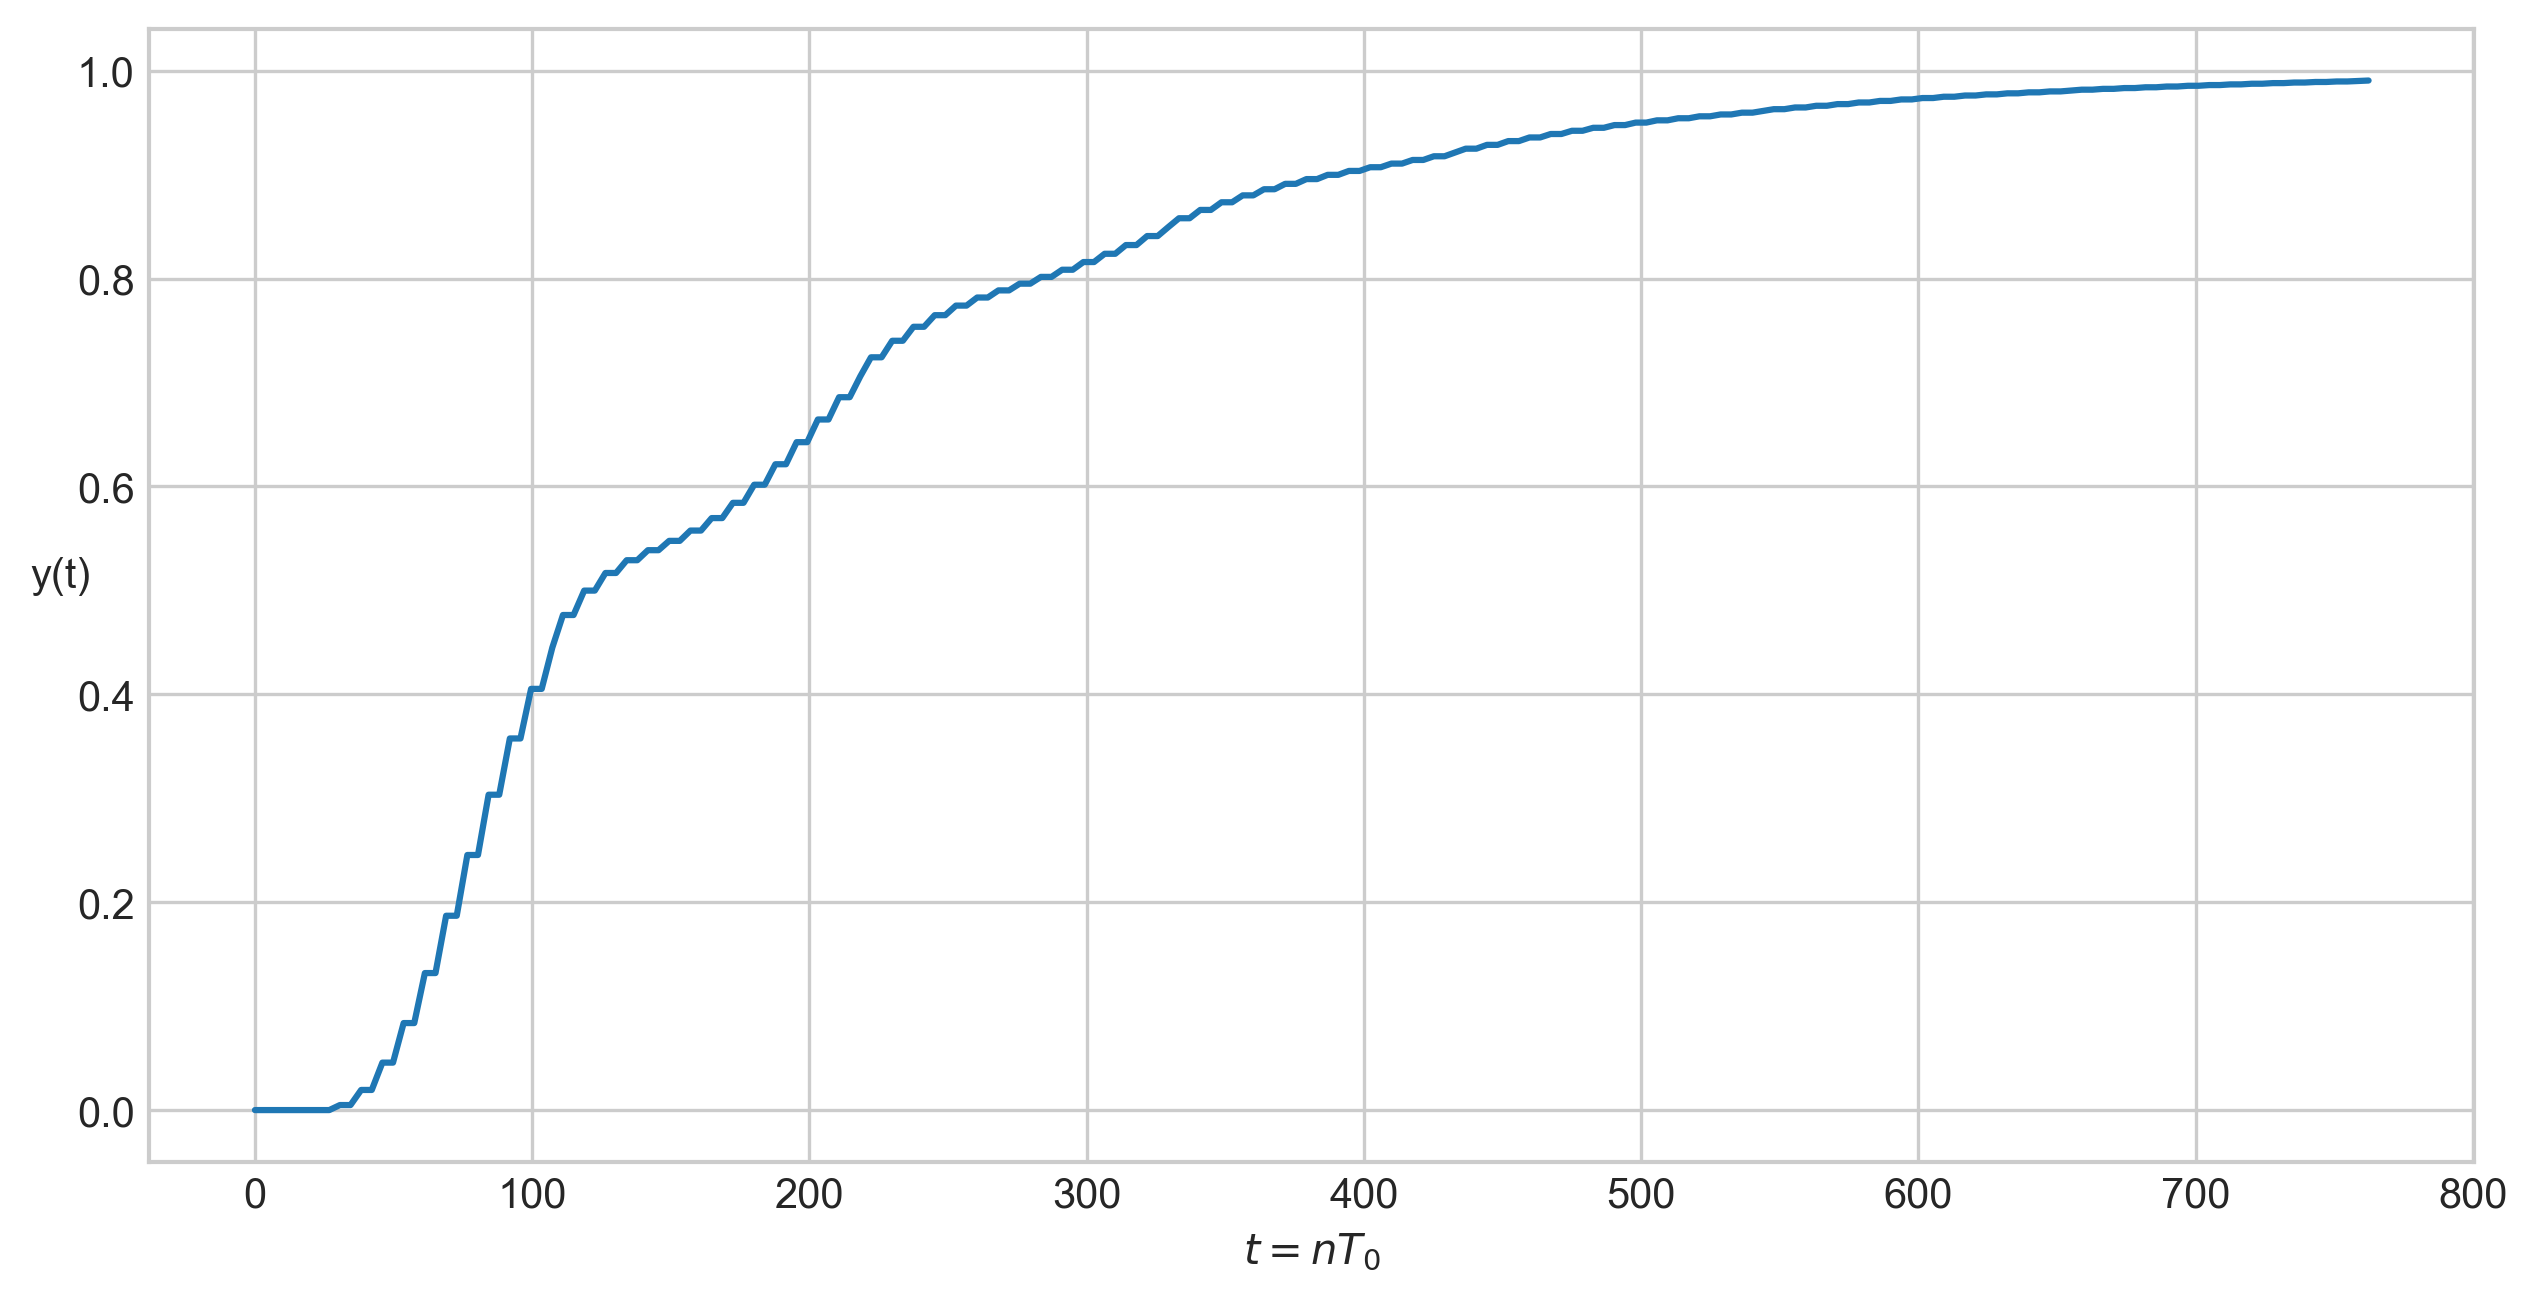
\includegraphics[scale=0.7]{pics/transient_process_final_9_2_step.png}
% \end{center}

\section{Випадок 
\texorpdfstring{$W_O(s) = \frac{ k e^{-\tau s}}{T_1 s + 1}$}{1}}
Оптимальні настройки регулятора для різних значень параметра $\lambda$ 
було обчислено в розділі \ref{ch:direct}.
Зв'язок між вихідною координатою та керуючим діянням задається диференціальним рівнянням
\begin{gather*}
    \mbox{\normalsize 
    $T_1 \frac{d y(t)}{dt} + y(t) = k u(t-\tau)$
    }
\end{gather*}
% Перехідні процеси при подачі на задаюче діяння одиничного імпульсу:
% \begin{center}
%     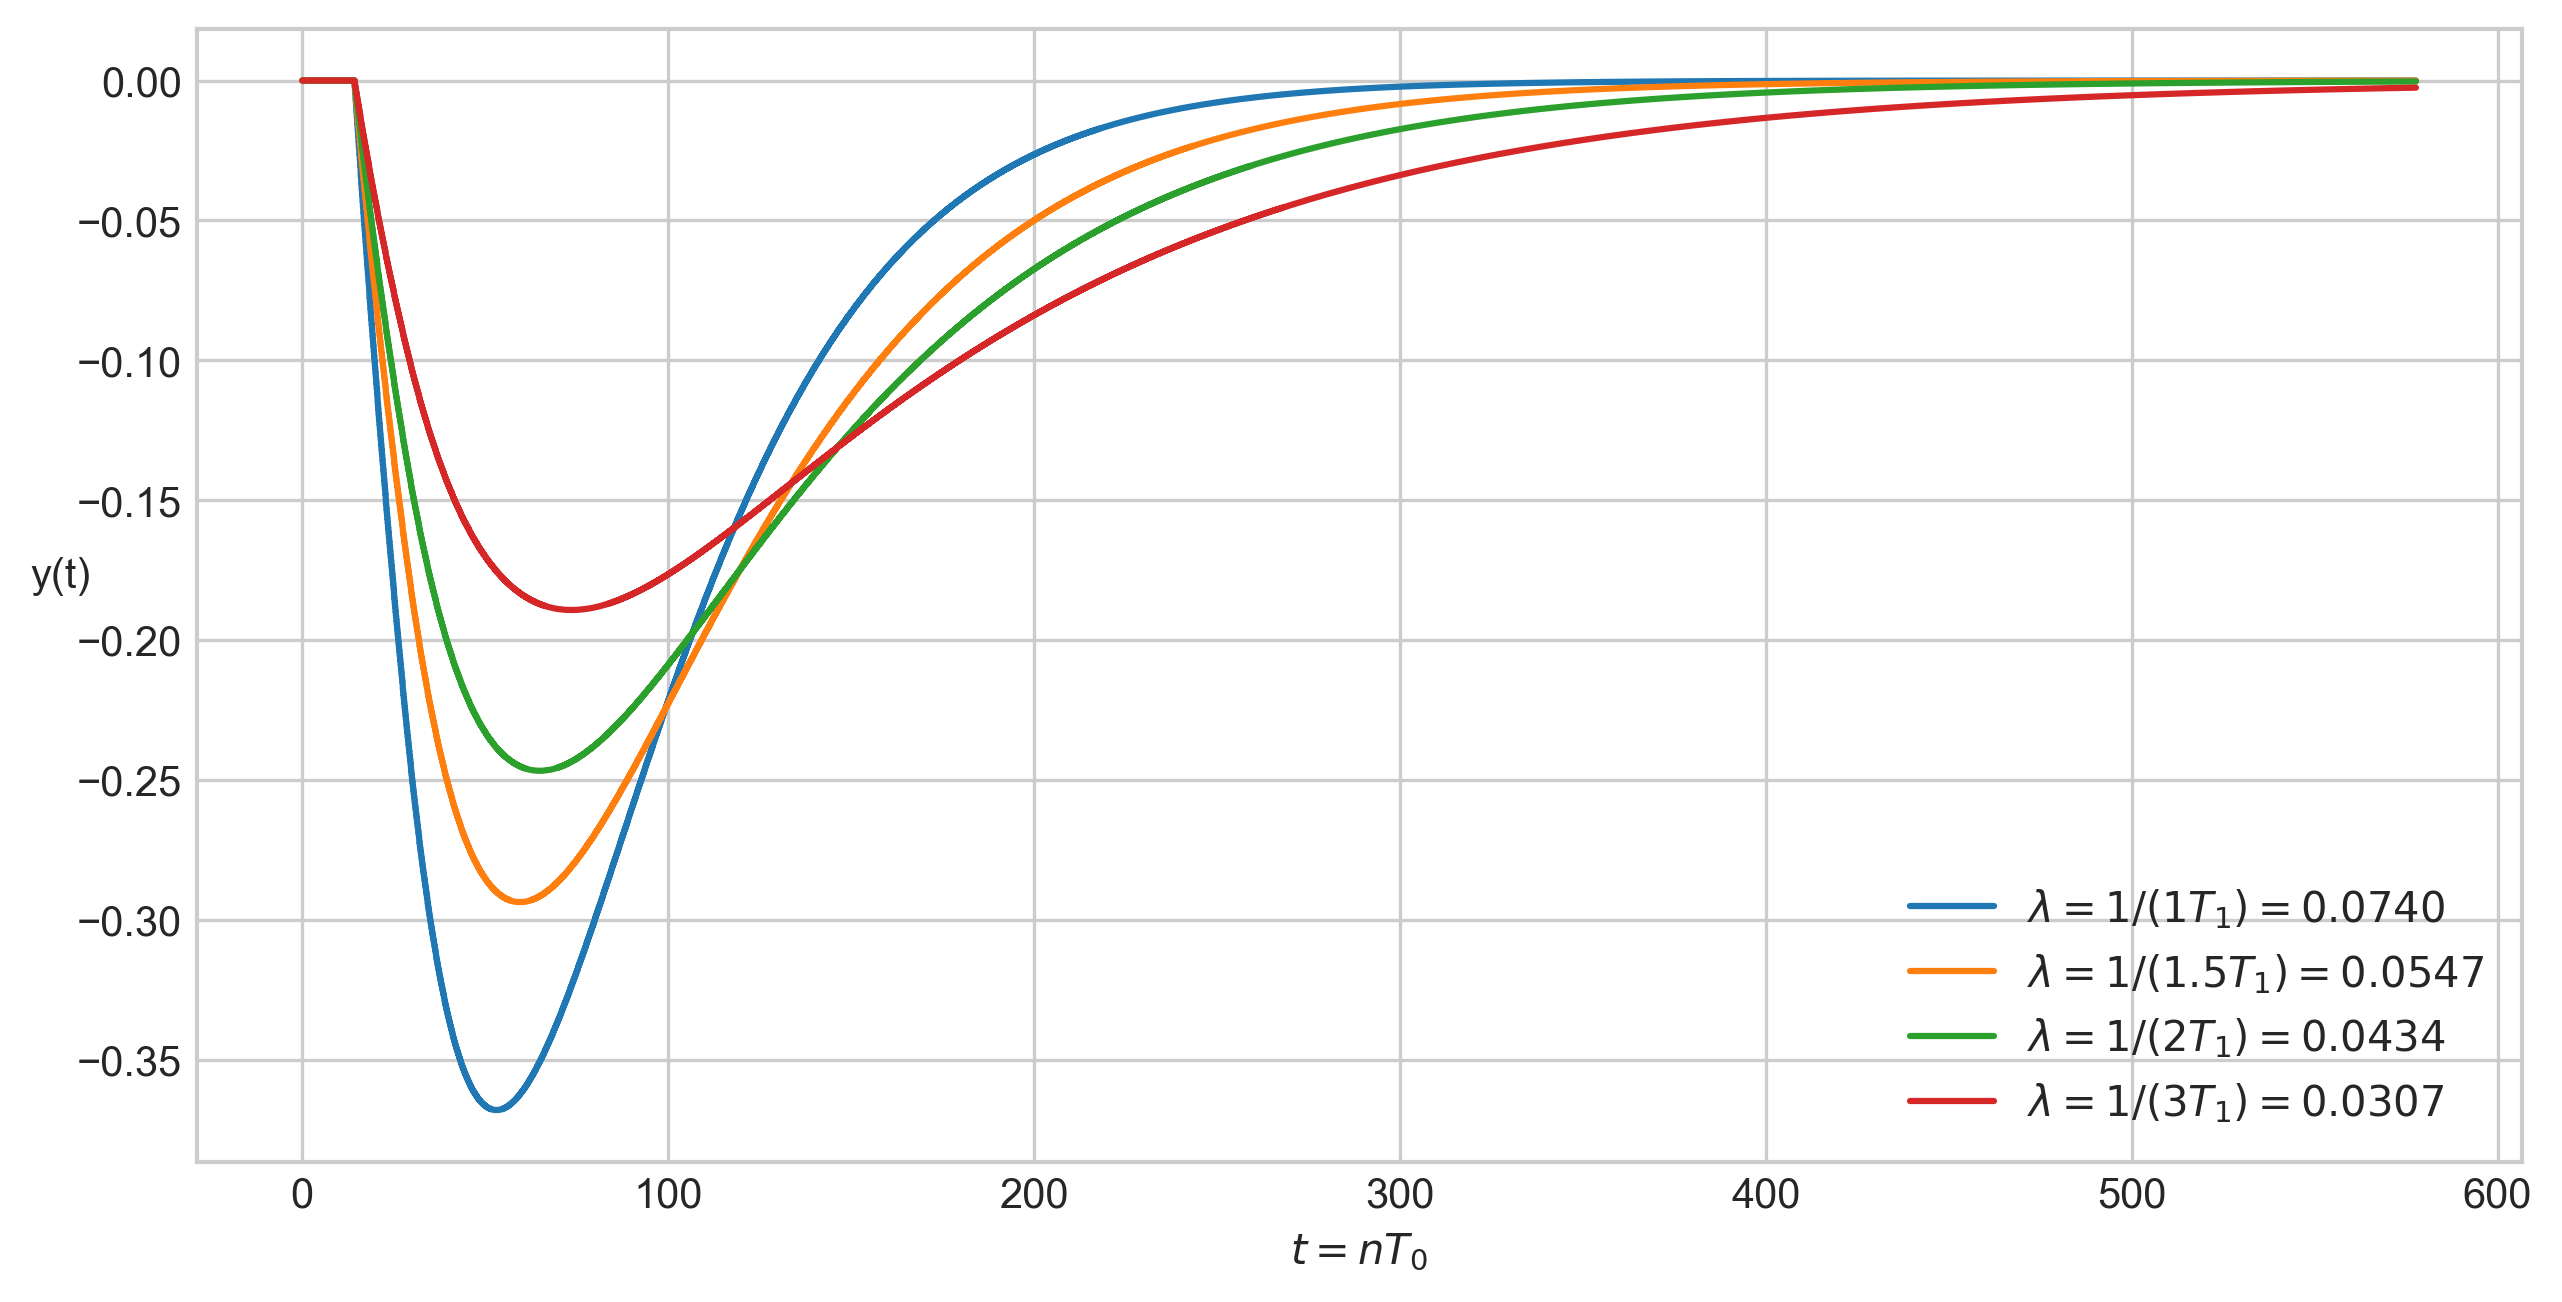
\includegraphics[scale=0.7]{pics/transient_process_final_9_3_impulse.png}
% \end{center}
Перехідні процеси при подачі на задаюче діяння одиничного ступінчатого збурення:
\begin{center}
    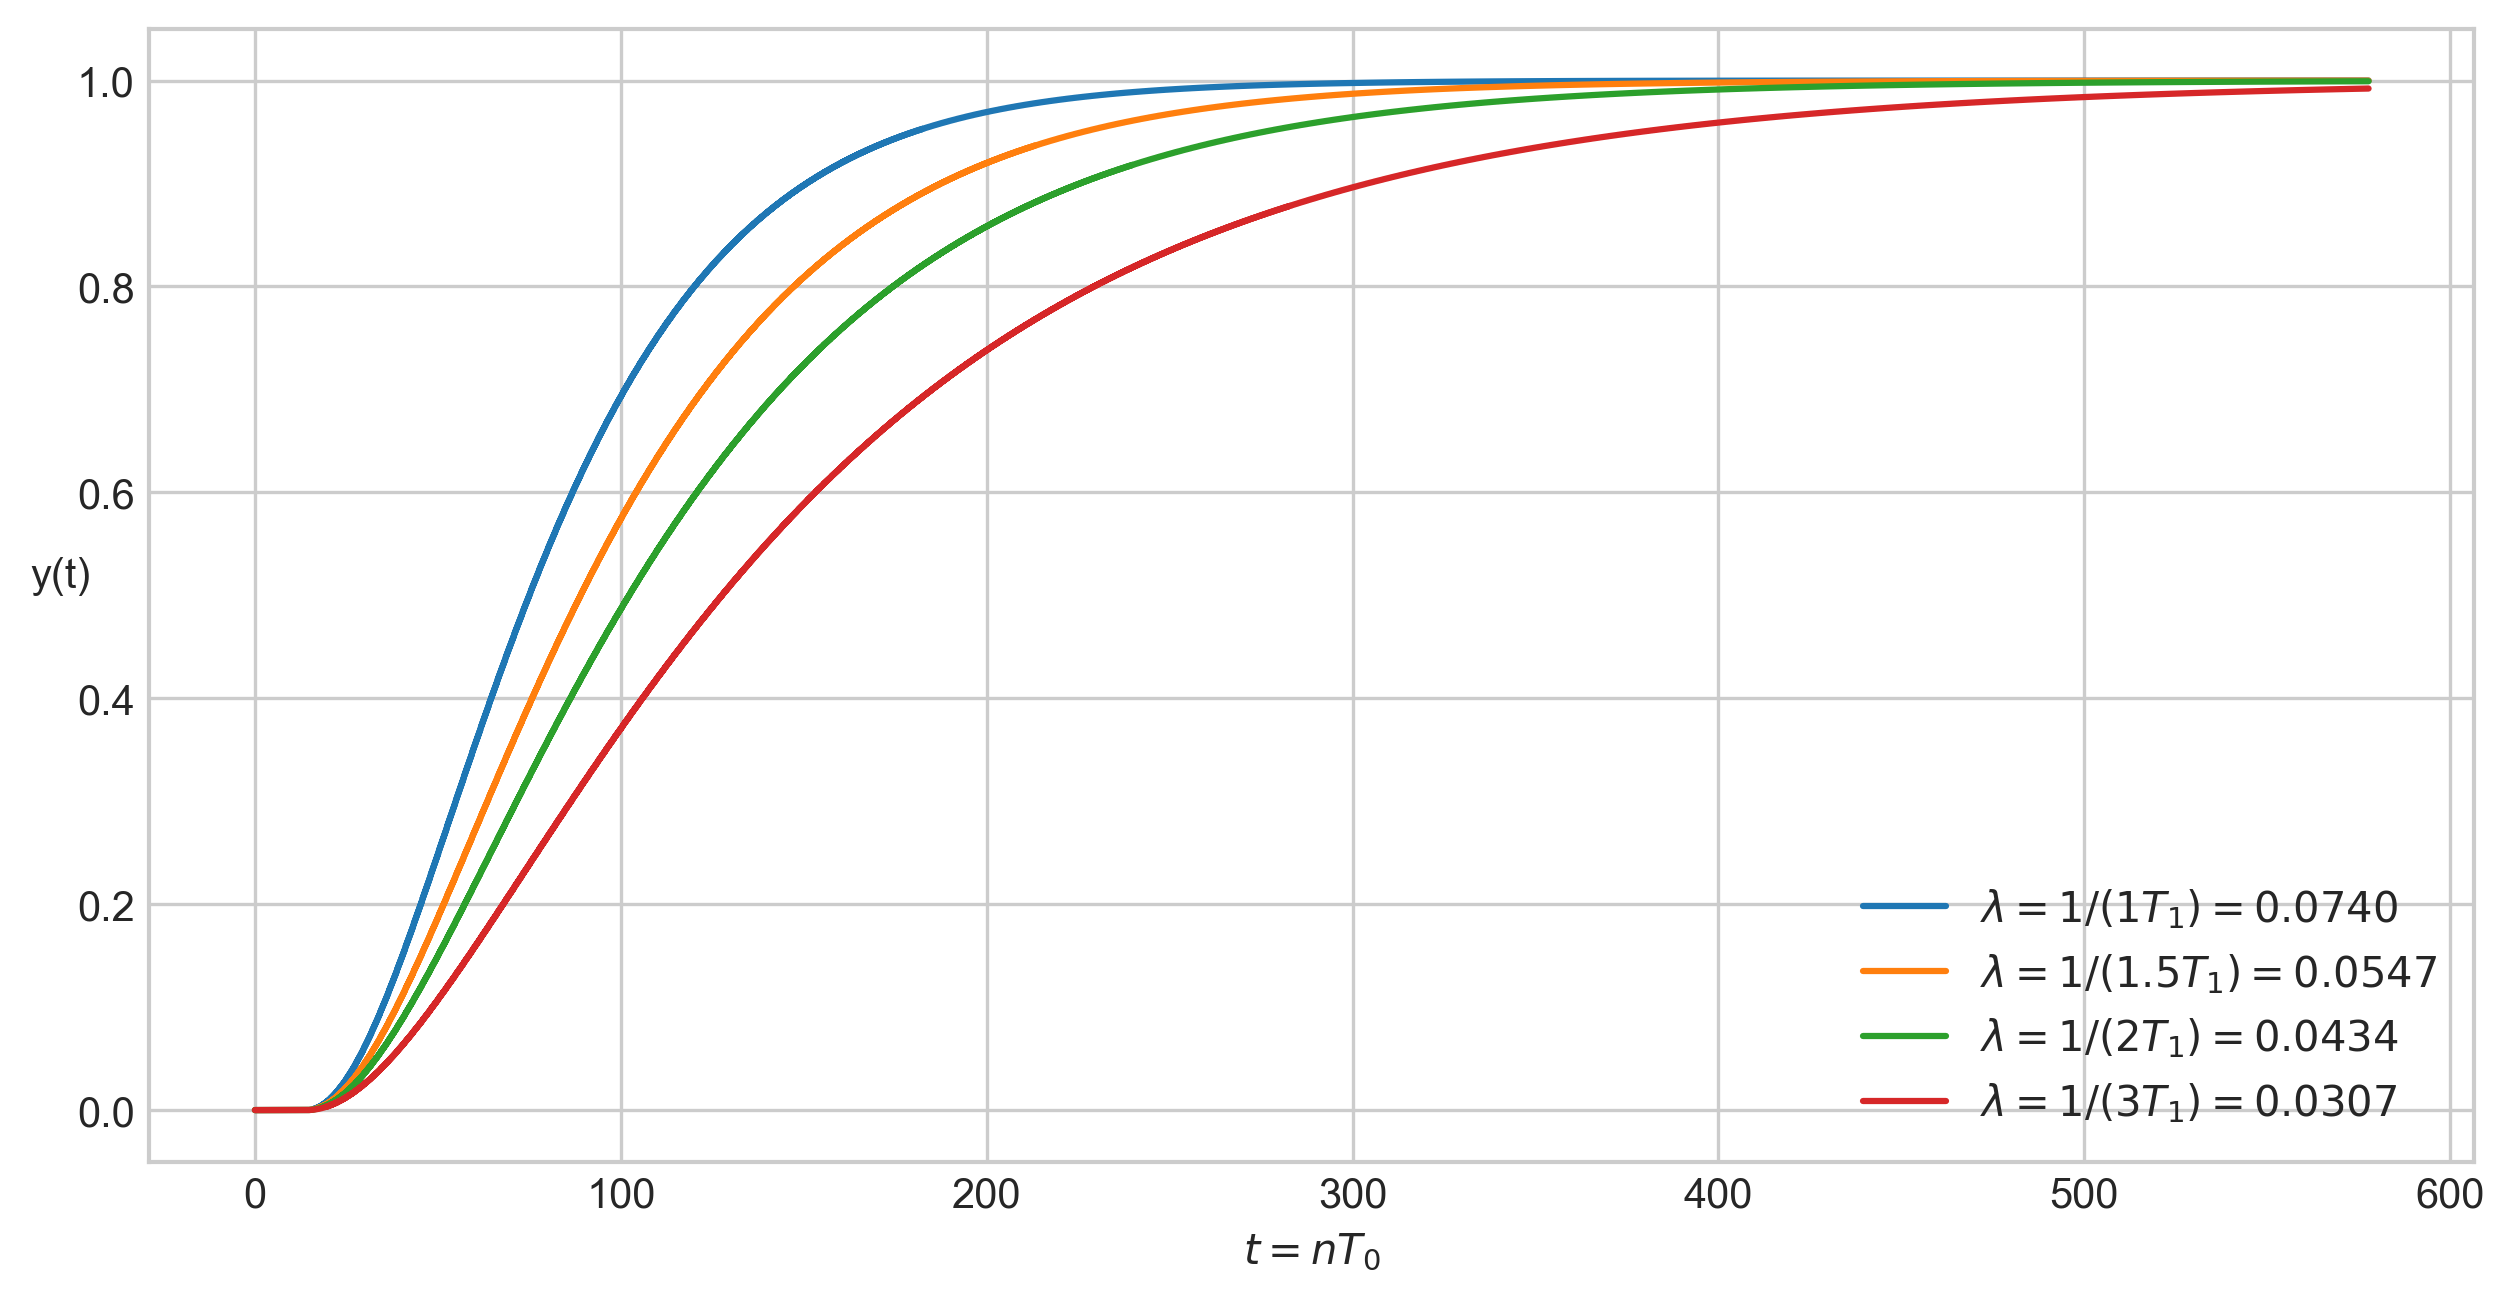
\includegraphics[width=\textwidth]{pics/transient_process_final_9_3_step.png}
\end{center}